\chapter{Thermal-Mechanical Design}  \label{thermal}

\section{Thermal Requirements}
Discuss requirements for the electronics before going into more detail in the self-emission section.

\subsection{Optical System}
The major thermal requirement driving the design for the LIFE instrument is the optical system. A Computer Assisted Design (CAD) model of the optical system is shown in Figure \ref{fig:optical_system_diagram}.

\begin{figure}[h]
\centering
  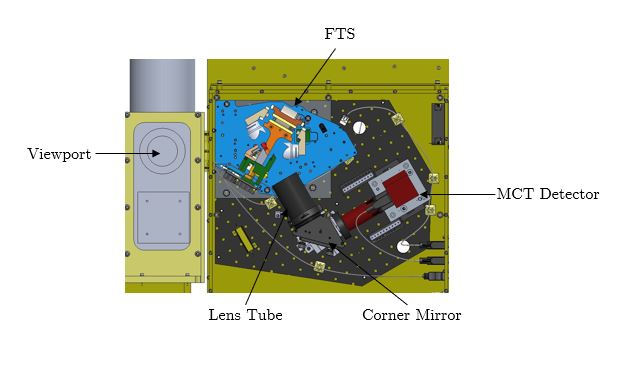
\includegraphics[width=\linewidth]{chap4_images/optical_system_diagram.JPG}
  \caption{LIFE optical system model}
  \label{fig:optical_system_diagram}
\end{figure}

The optical system consists of the FTS, the MCT detector, and the imaging lens system between the FTS and detector. The detector must be operated at 70K or lower, which is taken care of by its built-in Stirling cooler, so this did not need to be considered in the analysis. However, the impact of the heat radiated by the cooler on the rest of the system was considered. The lens array and FTS are the parts that need to be most carefully controlled. To prevent condensation on the lenses, the lower temperature requirement was set at 10°C. This provides a reasonably large margin so that the optics do not drop close to 0°C. To prevent any thermal expansion on the lenses and to protect to the FTS, the upper temperature limit was set to be 25°C. Further, inside this temperature range, the FTS and lens temperatures need to be as steady as possible over short time frames (i.e. less than 0.1°/min) as to not cause high thermal drift, which would have a detrimental effect on the measurements. 

\subsection{Electronics}
Various electrical components of the detector system have stringent operational temperature requirements. It is typical to place electronics in a separate box from the optical system, but the temperature must still be carefully controlled in order to prevent freezing or overheating of the electronics components. The most thermally sensitive components are the control board for the FTS system (BMXS Board), and the ethernet interface boards (Pleora Boards) attached to the detector data acquisition boards. The thermal requirements for the most thermally delicate components of LIFE are detailed in Table \ref{therm_req_table}. 

\begin{table}[h]
\begin{center}
\begin{tabular}{ |c|c|c|c| }
 \hline
 \rowcolor{lightgray}
 Component & Location & Minimum & Maximum \\
 \rowcolor{lightgray}
  &  & Temperature (°C) & Temperature (°C) \\
  \hline
  \hline
 Lens Array & Optics Box & 10 & 25 \\
 \hline
 FTS & Optics Box & 10 & 35 \\
 \hline
 BMXS Board & Electronics Box & 5 & 35 \\
 \hline
 Pleora Board (x2) & Electronics Box & 0 & 40 \\
 \hline
 Motor Driver & BB Electronics Box & 0 & 70 \\
 \hline
\end{tabular}
\end{center}
\caption{Temperature limits of most thermally delicate LIFE components that drive the thermal design}
 \label{therm_req_table}
\end{table}

These requirements must be considered in both the cold scenario and the warm scenario. The electrical components of LIFE, especially the detector data acquisition boards, dissipate a total power upwards of 500 W. The instrument must be designed so that in the lab, the instrument will not overheat and is able to dissipate this heat. In the cold case, even though the instrument is dissipating a high amount of power, it will still become too cold during flight. Heaters must be added to ensure that the delicate components of the instrument do not drop below zero during the float period. These heaters must also keep the temperature of the optical components steady; as discussed previously, they cannot fluctuate rapidly while the instrument is operational. 

\subsection{Mechanical}
Discuss the CSA requirements for the mechanical design, such as the size restraints, the bolt
holes and the forces on impact
[TODO]

\section{Thermal Environment}
Discuss temperatures the instrument will see, especially from CATS flight. There are subsubsections for each part of this section as much of it is explained in the background - ensure that what is discussed here relates specifically to the instrument design (the surface chosen and how it relates to emissivity, for example).

\subsubsection{Lab Environment}
Briefly talk about what the instrument will see in the lab, and why fans were implemented. May not be worth its own subsection.
[TODO]

\subsubsection{Ascent}
Talk about convection and rapidly varying temperatures seen on the ascent of the instrument.
[TODO]

\subsubsection{Float}
Conduction at altitude.
[TODO]

\section{Thermal Simulation Software}
To meet these numerous temperature requirements, a thermal model was created based on a mechanical model and was used for simulations of the hot and cold vacuum environments the instrument would face. The mechanical design could then be iterated based on the thermal simulation results. Numerous software packages were examined to determine the best simulation software to create and simulate the thermal model. In the end, the best and most convenient choice was to use the thermal analysis package as part of the SolidWorks CAD software. SolidWorks was used for the mechanical design for LIFE, so it was convenient to prepare the model for thermal design.

\subsection{SolidWorks}
Talk about SolidWorks a bit (may be discussed a bit in the mech section if that stays in there).
[TODO]

\subsection{FEA}
The first step in Finite Element Analysis (FEA) is to create a mesh, i.e. a finite number of spatial grid points, that span the model. This mesh is the combination of many very simple shapes, most often some type of triangle, to span an originally complex shape. These ‘finite elements’ combine to create a mesh, which has solution points on all vertices upon which these elements are connected. A set of algebraic equations are then created by using a numerical estimation to the various heat flux equations. For each node or vertex in this mesh, there is one simultaneous equation. 

\subsection{Solving simulations}
The SolidWorks thermal analysis software uses Finite Element Thermal Analysis to solve simulations, and considers heat flux due to heat power, radiation, conduction and convection. The unknown in these equations is the temperature. The restraints on these equations are the specified temperatures (for example, the baseplate must be -40°C as a worst-case scenario), and the reactions are the resultant heat flow that is necessary to maintain the specified temperatures. All other conditions add source terms, such as the dissipated heat power of electrical components~\citep{FEA_SW}.

For thermal equilibrium, the resulting matrix equations have a general form as shown in Equation \ref{gen_FEA_matrix}.

\begin{equation} \label{gen_FEA_matrix}
\begingroup \boldmath
    \begin{bmatrix}
        K_{uu} & K_{ug} \\
        K_{gu} & K_{gg}
    \end{bmatrix}
    \begin{bmatrix}
        T_u \\
        T_g \\
    \end{bmatrix}
    =
    \begin{bmatrix}
        F_g \\
        F_u \\
    \end{bmatrix}
\endgroup
\end{equation}

where $\bm{T_f}$ represents the restrained vertex temperatures and $\bm{F_g}$ represents the thermal heat power (heat flow) of the vertex. The $\bm{K}$ values represent the thermal conductivity matrix for each node, where if the material is assumed isotropic will be a unit matrix. $\bm{F_g}$ is unknown and represents the total heat flow in or out of a node that is necessary to maintain the given temperatures $\bm{T_g}$. $\bm{F_u}$ is calculated with heat flux, which is where conduction and radiation equations are used in the solution. For thermal conductive heat flux, Fourier's Law is used, from Equation \ref{FC_law}. Heat flux incident on the body and radiation from the body is from Equation \ref{SB_surroundings}. $\bm{F_u}$ is thus calculated from adding the conductive flux from Equation \ref{FC_law} the radiation flux from Equation \ref{SB_surroundings}, and the flux resulting from $\bm{F_g}$. This allows to complete the goal of the equations which is to solve for $\bm{T_u}$~\citep{FEA_SW}~\citep{FEA_Procedures}.

The size of the set of equations that is in general given by Equation \ref{gen_FEA_matrix} is the number of nodes. Thus, for an example of 100,000 nodes, there are 100,000 equations, and 100,000 temperatures calculated. Putting all these nodes together on the CAD model gives a solved thermal model necessary for thermal analysis.  The model can be evaluated for both lab and flight conditions by including or neglecting convection respectively, and by specifying relevant boundary conditions. 

\section{Pre-Flight Thermal-Mechanical Analysis \& Design}
Discuss all thermal analysis work done in terms of design to prepare for the flight. Can mention the verifications to the mech design in this section too (such as mechanical load simulations for the baseplate).

\subsection{Optics Box}
Discuss versions of the optics box thermal design.

\subsection{Electronics Box}
E-box thermal design versions.

\subsection{Full model}
Different versions of full model.

\subsection{TVAC Tests}
Results of the TVAC tests.

\subsection{Final Simulations}
Updates to simulations based on the TVAC tests.